\documentclass[11pt,a4paper]{article}
\usepackage[T1]{fontenc}
\usepackage[utf8]{inputenc}
\usepackage{lmodern,microtype}
\usepackage[margin=24mm]{geometry}
\usepackage{amsmath,amssymb,booktabs,graphicx,caption,float,tabularx,array}
\usepackage{xcolor,enumitem,fancyhdr}
\usepackage[hidelinks]{hyperref}
\definecolor{navy}{HTML}{174A6E}
\usepackage{titlesec}
\titleformat{\section}{\large\bfseries\color{navy}}{\thesection}{.65em}{}
\titleformat{\subsection}{\normalsize\bfseries}{\thesubsection}{.6em}{}
\setlength{\parindent}{0pt}\setlength{\parskip}{5pt}
\renewcommand{\topfraction}{.9}
\renewcommand{\textfraction}{.08}
\renewcommand{\floatpagefraction}{.8}
\setlength{\emergencystretch}{2em}\renewcommand{\arraystretch}{1.12}
\captionsetup{font=small,labelfont=bf}
\setlist{noitemsep,topsep=4pt,leftmargin=*}
\pagestyle{fancy}\fancyhf{}
\fancyhead[L]{\small Station08: temperature trends}
\fancyhead[R]{\small Computational Methods in Econometrics}
\fancyfoot[C]{\thepage}\renewcommand{\headrulewidth}{.3pt}
\setlength{\headheight}{14pt}
\graphicspath{{figures/}}
\newcommand{\degC}{\ensuremath{^{\circ}\mathrm C}}
\newcommand{\iid}{\mathrel{\mathop{\sim}\limits^{\mathrm{iid}}}}
\newcommand{\Nobs}{226}
\newcommand{\FirstYear}{1753}
\newcommand{\LastYear}{2013}
\newcommand{\NMissing}{35}
\newcommand{\MeanYear}{1866.4071}
\newcommand{\YMean}{9.5034}
\newcommand{\YSd}{0.6958}
\newcommand{\YMin}{7.6483}
\newcommand{\YMax}{11.7300}
\newcommand{\LinearIntercept}{9.4481}
\newcommand{\LinearSlope}{0.0337}
\newcommand{\DWstat}{1.4147}
\newcommand{\DWLower}{1.7549}
\newcommand{\DWUpper}{2.2695}
\newcommand{\DWp}{0.0002}
\newcommand{\BPstat}{0.4173}
\newcommand{\BPp}{0.5183}
\newcommand{\BreakYear}{1851}
\newcommand{\BrokenIntercept}{9.0690}
\newcommand{\PreSlope}{-0.0525}
\newcommand{\DeltaSlope}{0.1412}
\newcommand{\PostSlope}{0.0887}
\newcommand{\BreakStat}{12.2106}
\newcommand{\SigmaHat}{0.6182}
\newcommand{\Reduction}{12.5305}

\begin{document}
\begin{titlepage}\thispagestyle{empty}\vspace*{20mm}
{\color{navy}\LARGE\bfseries Temperature trends at Station08\par}
\vspace{6mm}{\Large Linear trends, structural change, and bootstrap inference\par}
\vspace{12mm}{\large Computational Methods in Econometrics\par}
Vrije Universiteit Amsterdam\par Academic year 2026--2027\par
\vspace{12mm}\textbf{Data:} Station08.csv, \FirstYear--\LastYear, \Nobs\ observed years\par
\textbf{Analysis date:} 28 September 2026\par
\vspace{12mm}\textbf{Abstract}\par
This study examines the annual temperature record of Geneva, Switzerland, supplied as Station08. A single linear trend rises by 0.0337\,\degC\ per decade, but its residuals show substantial dependence. A continuous broken trend fits best at 1851 and lowers the residual sum of squares by 12.5\%. Its slopes are $-0.0525$ and $0.0887$\,\degC\ per decade before and after that date. A calendar-aware dependent wild bootstrap gives a break-test $p$-value of 0.0331; increasing the dependence bandwidth changes it to 0.0541. Both bootstrap interval constructions include zero for the pre-break slope and exclude it for the post-break slope. An 8,000-dataset simulation finds severe over-rejection by independent-error bootstrap methods under serial correlation, while the dependent wild procedure is conservative. The evidence supports a rising later trend and a useful change in fitted slope, with qualified evidence about an unknown structural break. Missing years, incomplete measurement-history information and the single-break specification limit interpretation.
\vfill\small All estimates, figures and simulation results follow the refined \texttt{main.Rmd}. The report retains all 226 supplied observations and uses the supplied station metadata. The data source is the quality-controlled, homogenisation-adjusted GHCN-M v4 Geneva series.
\end{titlepage}\pagenumbering{arabic}

\section{Introduction and research question}
Does the record at Station08 reveal sustained warming, and does a constant linear trend adequately describe its evolution? A positive fitted slope alone cannot answer this question. Annual temperatures fluctuate, residual dependence changes the uncertainty of trend estimates, and a single slope may average over different historical patterns. We begin with a descriptive linear fit, assess its residuals, and compare it with a continuous model whose slope changes at an unknown date. A simulation study evaluates the inferential procedures under known data-generating processes.

The empirical object is the Geneva station series, rather than regional or global climate. We estimate changes in annual mean temperature, not a causal effect of a specific driver. The supplied metadata identifies the station and data product, but does not resolve all measurement-history changes or establish broader representativeness. The project follows the assignment's linked tasks: diagnostics, bootstrap inference about structural change, and Monte Carlo evaluation \cite{handout}.

\section{Data and exploratory analysis}
\subsection{Station, sample and missing years}
Station08 is Geneva, Switzerland, at $46.20^\circ$N, $6.15^\circ$E and 405\,m elevation. The supplied metadata identifies NOAA NCEI's Global Historical Climatology Network Monthly Temperature dataset, version 4 (GHCN-M v4), QCF adjusted series. Annual means require at least ten valid monthly observations \cite{menne,stationdata}. The QCF data are quality controlled and homogenisation adjusted: pairwise homogenisation aims to remove artificial shifts due to changes such as station relocations and instruments. This reduces such concerns but cannot establish that every remaining change is climatic. Early records have fewer neighbouring observations for comparison, and residual inhomogeneities remain possible.

The CSV contains \Nobs\ unique observations between \FirstYear\ and \LastYear, with numeric columns \texttt{Year} and \texttt{Temperature}, no missing cells and no duplicated years. After sorting and validation, we retain every supplied observation and do not transform temperature. There are nevertheless \NMissing\ missing calendar years across five gaps (Table~\ref{tab:gaps}). Absence of missing cells is not an uninterrupted annual record. We neither interpolate gaps nor discard observed years.

\begin{table}[htbp]\centering\small
\caption{Missing years between consecutive supplied observations. The complete range contains 261 calendar years and 226 observed temperatures.}\label{tab:gaps}
\begin{tabular}{rrrr}\toprule
Last observed year & Next observed year & Missing interval & Missing years\\\midrule
1930 & 1932 & 1931 & 1\\
1967 & 1969 & 1968 & 1\\
1972 & 1976 & 1973--1975 & 3\\
1978 & 1980 & 1979 & 1\\
1980 & 2010 & 1981--2009 & 29\\\bottomrule
\end{tabular}\end{table}

Observation adjacency therefore differs from calendar adjacency. In particular, 1980 and 2010 are 30 years apart. Observed-data lines stop across gaps; fitted curves and variance smooths inside them are model-implied, not observations. The four final values cannot show whether warming during the missing decades was gradual, accelerating or interrupted, and their difference from 1980 is not evidence of a discontinuity.

\subsection{Exploratory features and time index}
The sample mean is \YMean\,\degC\ and its standard deviation is \YSd\,\degC. The coldest observation is \YMin\,\degC\ in 1851 and the warmest is \YMax\,\degC\ in 2011. Means are 9.49\,\degC\ before 1800, 9.20 in 1800--1849, 9.26 in 1850--1899 and 9.79 in 1900--1980. All four observations in 2010--2013 are among the twelve warmest. The record drifts downward into the mid-nineteenth century and rises thereafter (Figure~\ref{fig:series}); this motivates examining a changing slope.

Year-to-year variation is substantial relative to this slow movement. The raw standard deviation is 0.665\,\degC\ before 1900 and 0.610\,\degC\ thereafter. These measures include within-period trend movements, so they are descriptive rather than tests of changing error variance. No extreme observation is removed; the role of the coldest year is examined separately.

We distinguish observation position $i=1,\ldots,n$ from calendar year $s_i$ and use
\begin{equation}
 x_i=(s_i-1850)/10.\label{eq:time}
\end{equation}
One unit is one decade, so slopes have units \degC\ per decade. Calendar spacing enters the regression even when years are missing. Centring at 1850 changes the intercept but leaves fitted values, residuals, slopes and test statistics unchanged. This reference year was chosen for presentation after seeing the estimated break near 1850; it carries no inferential weight. Appendix~\ref{app:centring} explains the intercept interpretation. Trimming operates on observation positions, as specified in the assignment.

\begin{figure}[htbp]\centering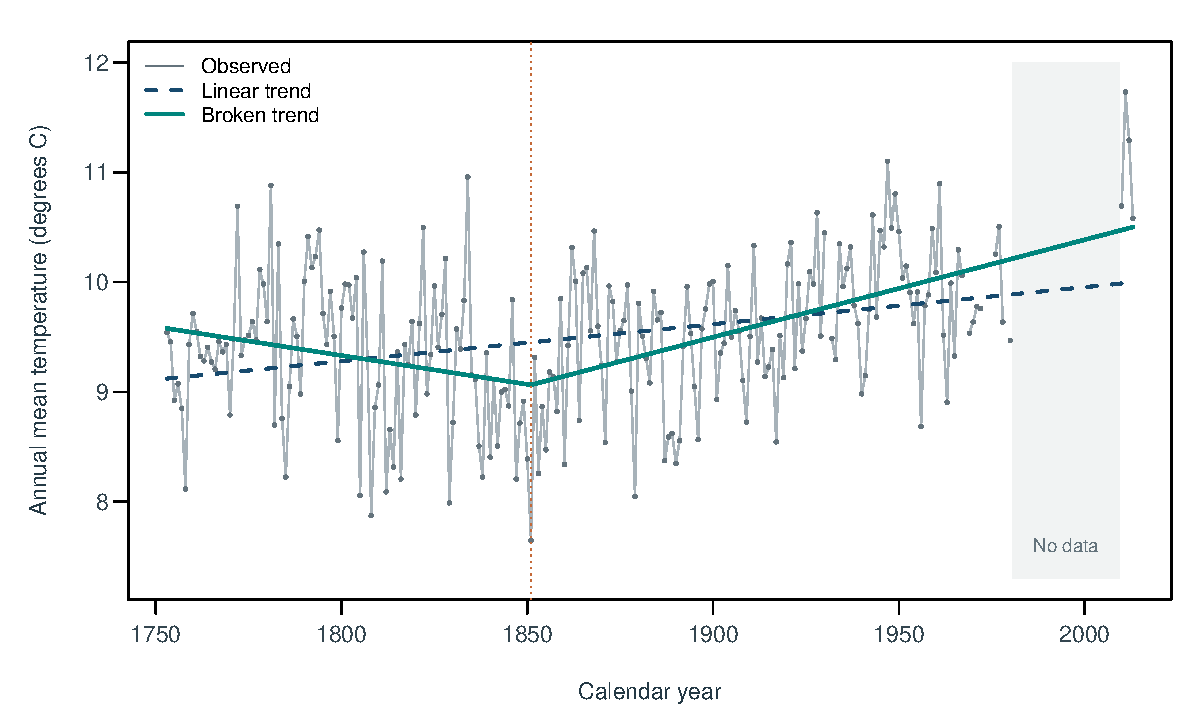
\includegraphics[width=.96\linewidth]{temperature_fits.pdf}
\caption{Observed annual temperatures and fitted models using all 226 observations. Observation lines stop across missing years. The shaded interval contains no observations; fitted curves across it are model-implied. The vertical line marks the best-fitting break at 1851.}\label{fig:series}\end{figure}

\section{Linear trend and model diagnostics}
\subsection{Estimation and residual plots}
OLS in $y_i=\beta_0+\beta_1x_i+\varepsilon_i$ gives
\begin{equation}\widehat y_i=\LinearIntercept+\LinearSlope x_i.\end{equation}
The intercept is the fitted temperature in 1850. Because the reference year differs from the mean observed year, it does not equal the sample mean. The slope corresponds to approximately 0.337\,\degC\ per century, or 0.876\,\degC\ across the 260-year span. These are descriptive changes under a constant-trend approximation, not significance statements. The fit explains only 10.5\% of total variation; annual variability remains large. OLS is well defined on this fixed, irregular calendar design, but the gaps affect which periods inform the estimate and its precision. The 222 observations through 1980 also inform the slope; it is not solely a comparison with the final four. Neither exogeneity nor the missing-year mechanism can be verified from these data, and the fitted line does not recover the unobserved trajectory.

The residual time plot in Figure~\ref{fig:linear-diagnostics} shows low-frequency departures and runs with the same sign. A residual is observed minus fitted temperature, so these runs suggest dependence or remaining structure in the mean. The observation-lag ACF(1) is 0.290, whereas the calendar-lag value is 0.302. For the latter, we place residuals on the full annual grid and insert \texttt{NA} for absent years; no temperatures are imputed. The estimates use available pairs, can fail to define a valid autocorrelation sequence, and their conventional reference bands are descriptive rather than calibrated inference. The similar first-lag values here do not make observation and calendar lags interchangeable.

The squared-residual plot and normal QQ plot appear in Appendix~\ref{app:linear-marginal}. The variance smooth has local rises and falls, including an increase near the final four observations; a narrow linear variance test can miss such patterns. The curve across the long gap is unsupported by observations there. The QQ plot is broadly linear in its centre with tail departures. It is a marginal descriptive comparison, not evidence of independence, and Gaussian errors remain an explicit reference assumption rather than a verified property.

\begin{figure}[htbp]\centering
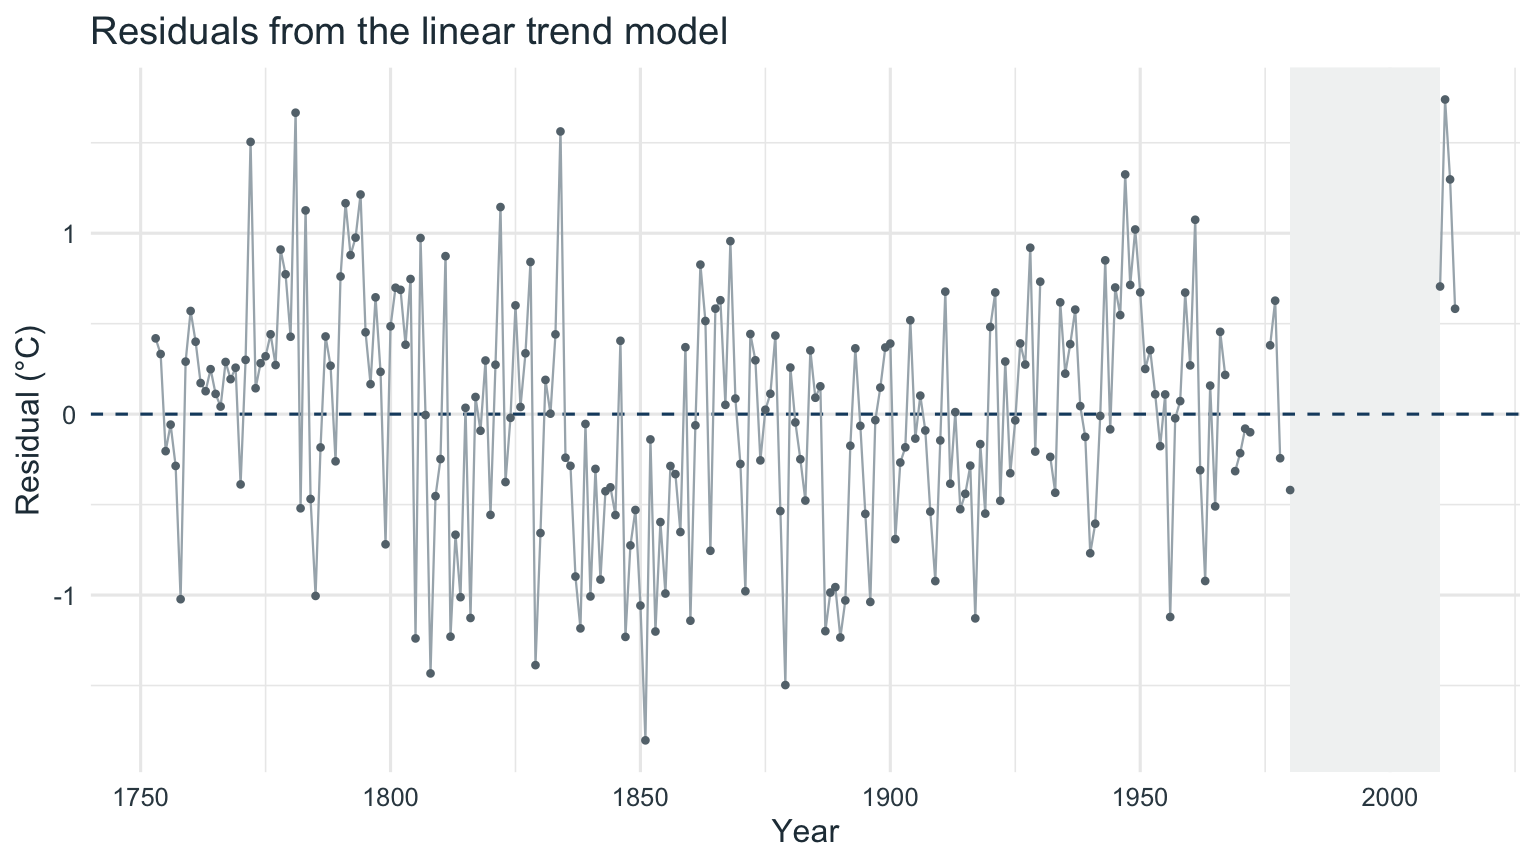
\includegraphics[width=.86\linewidth]{resid-time-plot-1.png}\\[2mm]
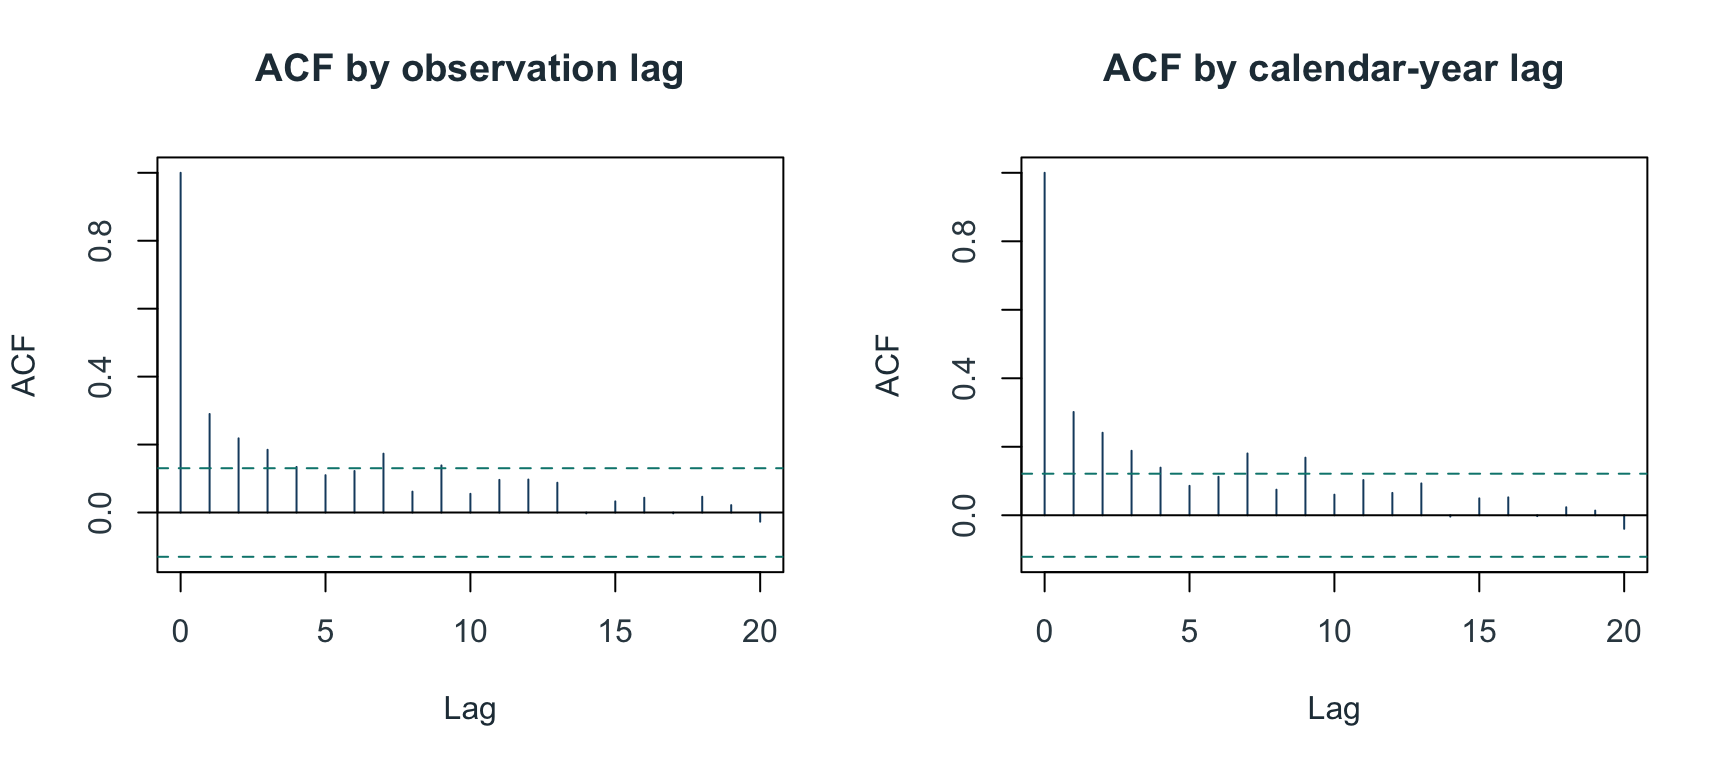
\includegraphics[width=.96\linewidth]{acf-compare-1.png}
\caption{Linear-model residuals against calendar year (top) and sample ACFs by observation lag and calendar-year lag (bottom). Observed lines stop at gaps. The calendar ACF uses an annual grid with missing years set to NA; its bounds, like the observation-lag bounds, are descriptive guides.}\label{fig:linear-diagnostics}\end{figure}

\subsection{Monte Carlo Durbin--Watson test}
The assignment's adjacent-observation statistic is
\begin{equation}\widehat d=\frac{\sum_{i=2}^n(\widehat\varepsilon_i-\widehat\varepsilon_{i-1})^2}{\sum_{i=1}^n\widehat\varepsilon_i^2}=\DWstat.\end{equation}
There are 225 adjacent-observation pairs, of which 220 are consecutive calendar years. We implement the assigned statistic as the primary diagnostic of observation-adjacent dependence. Restricting its numerator to consecutive years defines a different statistic, retained as a sensitivity check:
\[
d_{\mathrm{calendar}}=
\frac{\sum_{i:\,s_{i+1}-s_i=1}(\widehat e_{i+1}-\widehat e_i)^2}
{\sum_i\widehat e_i^2}.
\]
Each version is calibrated using its own formula and the same simulated residual vectors. Under the conditional null of independent Gaussian errors with constant variance, draw $z^{(b)}\sim N(0,I_n)$ and calculate residuals $e^{(b)}=M_Xz^{(b)}$, where $M_X=I-X(X'X)^{-1}X'$ and $X=[\mathbf1,x]$. Recompute the statistic for $B=9,999$ draws. Regression coefficients disappear through $M_X$ and the common error scale cancels in $e'Ae/e'e$, where $A$ represents the chosen differences. Thus each statistic has a finite-sample null reference conditional on its known design and difference matrix. Both simulations use seed 20260926.

The two tails are calibrated separately without assuming symmetry around two. R type-6 empirical 2.5th and 97.5th percentiles are \DWLower\ and \DWUpper. With $B=9,999$, these are the 250th and 9,750th ordered simulated statistics. The nominal 5\% rejection region is
\[\widehat d<\DWLower\quad\text{or}\quad\widehat d>\DWUpper.\]
The equal-tail Monte Carlo $p$-value is
\begin{equation}
 p_{MC}=\min\left\{1,2\min\left[\frac{1+\sum_b\mathbf1(d^{(b)}\leq\widehat d)}{B+1},\frac{1+\sum_b\mathbf1(d^{(b)}\geq\widehat d)}{B+1}\right]\right\}=\DWp.
\end{equation}
Under the continuous iid Gaussian null, strict rejection outside the cutoffs agrees with $p_{MC}\leq0.05$. The rank rule has exact 5\% size for this replication count, although its realised simulated cutoffs and p-value vary across runs \cite{dufour}. It is not an exact test of every process with zero first-order correlation.

\begin{table}[htbp]\centering\small
\caption{Two-sided DW Monte Carlo tests using 9,999 common simulated residual vectors, separately calibrated for each definition.}\label{tab:dw}
\begin{tabular}{lrrrr}
\toprule
Definition & Statistic & Lower 2.5\% & Upper 97.5\% & $p$-value \\
\midrule
Observation adjacency (primary) & 1.4147 & 1.7549 & 2.2695 & 0.0002 \\
Calendar adjacency & 1.3865 & 1.7106 & 2.2211 & 0.0002 \\
\bottomrule
\end{tabular}
\end{table}

Both versions reject in the lower tail (Table~\ref{tab:dw}), indicating positive residual dependence relative to the iid Gaussian reference. Their p-values are at the attainable simulation floor, not zero probabilities. The optional \texttt{lmtest::dwtest} comparison also uses a two-sided alternative, but does not replace the Monte Carlo calibration. An inadequate linear mean can itself generate serially patterned residuals; rejection does not identify a physical or statistical cause.

\subsection{Breusch--Pagan diagnostic and inferential principles}
The auxiliary regression uses the same transformed regressor: $\widehat\varepsilon_i^2=\gamma_0+\gamma_1x_i+v_i$. We test $H_0:\gamma_1=0$ against $H_1:\gamma_1\neq0$. The requested statistic is $BP=nR^2=\BPstat$, with nominal $\chi^2_1$ $p$-value \BPp. Homoskedasticity is not rejected against a linear variance trend at 5\%. This does not establish homoskedasticity: the alternative is narrow, power is finite, and detected serial correlation weakens the usual chi-square calibration. We use the handout's $nR^2$ convention, the studentised form associated with Koenker \cite{koenker} of the Breusch--Pagan diagnostic \cite{bp}.

The DW comparison requires care. An iid Gaussian Monte Carlo reference is also possible for $BP$ if the complete null error model is specified. Nonlinearity in squared residuals does not prohibit simulation. However, homoskedasticity alone leaves the finite-sample distribution of squared residuals unspecified: higher moments and dependence matter. The requested chi-square reference is an asymptotic approximation under its regularity conditions, whereas the DW simulation specifies a spherical Gaussian null conditional on $X$. The BP statistic is scale invariant, but under a broad homoskedasticity null its finite-sample distribution still depends on the error-distribution shape, including fourth moments. Applying an iid Gaussian calibration to other distributions or serially dependent errors can distort size. The studentised asymptotic reference does not require normality under its regularity conditions. Neither procedure becomes distribution-free merely by removing coefficients and scale. Together, the diagnostics make independent-error inference difficult to justify, even though the variance-trend test does not reject.

\section{Structural change and bootstrap inference}
\subsection{A continuous trend with an unknown slope change}
For candidate observation $k$, define $h_{ik}=(x_i-x_k)_+$ and estimate
\begin{equation}y_i=\alpha+\beta x_i+\delta h_{ik}+\varepsilon_i.\label{eq:broken}\end{equation}
The pre-break slope is $\beta$, and the post-break slope is $\beta+\delta$. The hinge is zero at the break, enforcing continuity. Thus the model allows a slope change without an instantaneous level jump. At fixed $k$, the three regressors are known and OLS applies directly.

With 15\% trimming, the integer candidate set is $k=\lceil.15n\rceil,\ldots,\lfloor.85n\rfloor=34,\ldots,192$, corresponding to 1786--1945. Trimming protects against fits based on too few observations in a regime \cite{andrews}. We trim observation counts, not calendar duration: trimming 15\% of the calendar span could leave as few as eight observed years after a candidate because of the long gap. We fit every candidate, and minimum RSS selects $\widehat k=99$, or \BreakYear. Figure~\ref{fig:profile} displays the complete objective profile. The fitted equation is
\begin{equation}\widehat y_i=\BrokenIntercept\;\PreSlope x_i+\DeltaSlope(x_i-x_{99})_+.\end{equation}
The negative coefficient multiplying $x_i$ is the pre-break slope. The hinge is zero in 1850, so the intercept is fitted temperature in 1850, directly comparable to the linear intercept. It is not the fitted temperature at the break in 1851; that value is $\widehat\alpha+0.1\widehat\beta$. RSS falls from 97.447 to 85.237, giving
\begin{equation}F_T=RSS_0-\min_kRSS(k)=\BreakStat\quad(\degC^2).\end{equation}
Despite its label, $F_T$ is the handout's raw RSS reduction, not a variance-normalized $F$ ratio. The alternative is $\delta\neq0$ at some admissible date. The date is unidentified under $H_0:\delta=0$, and searching improves fit even in no-break data. Ordinary fixed-date tests do not calibrate this selection.

The selected year also contains the coldest observation. A continuous hinge describes a trough-shaped mean and can be attracted toward a pronounced local minimum; the sensitivity check therefore repeats the search without 1851. A mid-nineteenth-century turning point is consistent with conventional dating of the end of the Little Ice Age in the European Alps, where many glaciers reached their last maxima around 1850 \cite{matthews}. This agreement is suggestive only: one station and a fitted breakpoint cannot establish a regional transition or a cause.

\begin{figure}[htbp]\centering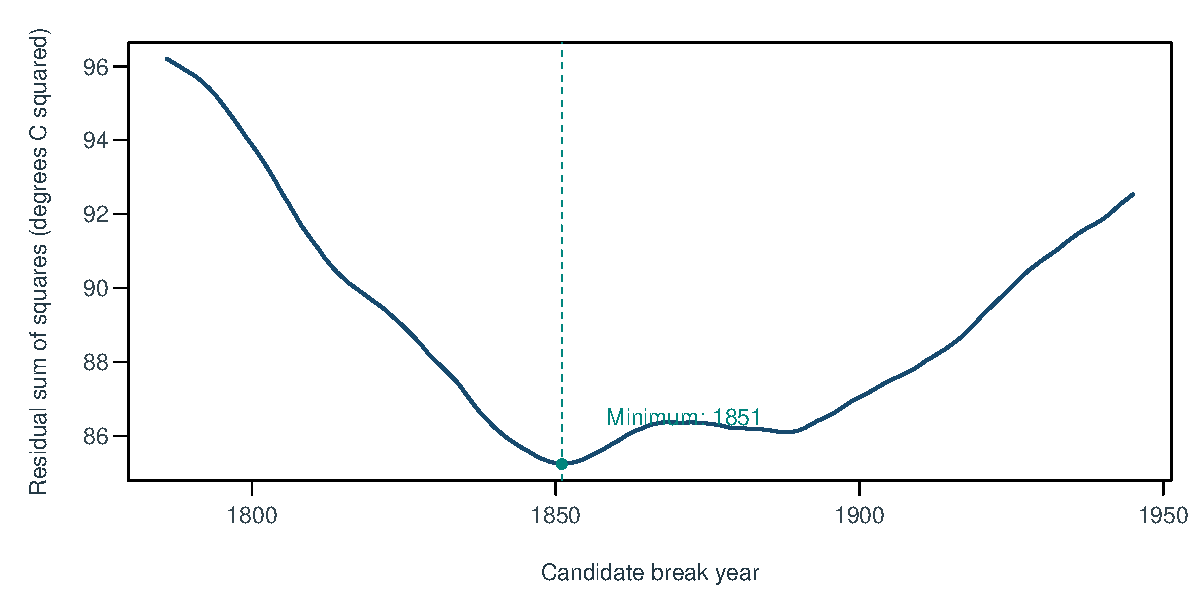
\includegraphics[width=.86\linewidth]{break_profile.pdf}
\caption{RSS over the trimmed candidate set. Its minimum identifies the best-fitting date; bootstrap inference determines whether the reduction is unusual under the no-break null.}\label{fig:profile}\end{figure}

\subsection{Bootstrap choices and complete testing algorithms}
The primary method is a dependent wild bootstrap (DWB) with Gaussian autoregressive multipliers evaluated at calendar gaps. It retains residual variance patterns while approximating short-range dependence. Dependent wild and autoregressive wild methods provide precedents for dependent, irregularly observed trend data \cite{shao,friedrich}. These motivate the construction but do not establish an exact guarantee for this particular unknown-break statistic. The simulation below evaluates finite-sample behavior in specified settings.

The diagnostics motivate preserving dependence: the primary DW p-value is 0.0002, while the conventional BP p-value of 0.5183 only concerns a linear variance trend and does not adjust for serial dependence. We also use an IID residual bootstrap and an independent wild bootstrap \cite{wu,liu}. The first targets independent, identically distributed errors; the second retains observation-specific residual scale but removes dependence. BP non-rejection does not rule out other variance patterns, so the wild procedure is a variance-robust sensitivity check. Comparing IID with wild assesses sensitivity to variance treatment; comparing wild with DWB assesses sensitivity to dependence treatment. These independent-error methods are not equally credible primary procedures after the diagnostics.

\textbf{Restricted residuals and bandwidth.} Testing samples are generated around the fitted null mean using restricted residuals. This targets $H_0$ but does not guarantee accurate finite-sample size. If the trend changes, restricted residuals may contain the unmodelled kink as low-frequency structure. Retaining more of that structure at longer bandwidths may raise critical values and reduce power, but p-values need not increase monotonically with bandwidth. Using broken-trend residuals while still generating around the null mean would change the calibration; its size and power effects would need a separate study.

The primary $\ell=6$ follows the $n^{1/3}$ rate. Its multiplier correlations are $\exp(-1/6)\approx0.85$ at one year, 0.37 at six years and 0.14 at twelve years. These are kernel correlations, not estimates of the residual ACF. Bandwidths three and twelve assess sensitivity to the retained dependence horizon.

For every method, the complete testing algorithm is:
\begin{enumerate}
\item Fit the no-break model and retain $\widehat y_{0i}$. Center its residuals and set $\widetilde e_i=(\widehat e_{0i}-\bar e_0)\sqrt{n/(n-2)}$, offsetting shrinkage from two estimated coefficients.
\item In the \textbf{IID residual} method, sample $n$ errors with replacement from $\{\widetilde e_i\}$. In the \textbf{independent wild} method, use $e_i^*=\widetilde e_iw_i$ with independent signs $w_i\in\{-1,1\}$ of equal probability. This retains each location's squared residual but removes cross-covariances.
\item In the \textbf{dependent wild} method, draw $w_1\sim N(0,1)$ and independent $z_i\sim N(0,1)$, and set
\[
 a_i=\exp[-(s_i-s_{i-1})/\ell],\quad w_i=a_iw_{i-1}+\sqrt{1-a_i^2}z_i,\quad e_i^*=\widetilde e_iw_i.
\]
The primary bandwidth is $\ell=\operatorname{round}(n^{1/3})=6$ years. The conditional covariance is $\widetilde e_i\widetilde e_j\exp(-|s_i-s_j|/\ell)$, approximating dependence while retaining the variance pattern. Multiplier correlation is not an estimate of error autocorrelation. Gaps reduce multiplier dependence without imputing temperatures.
\item Form $y_i^*=\widehat y_{0i}+e_i^*$. Refit the null and all candidate alternatives on the fixed original grid to obtain $F_T^*=RSS_0^*-\min_kRSS^*(k)$. Repeat $B=9,999$ times. The 95\% critical value is the type-1 empirical quantile; $p=(1+\sum_b\mathbf1\{F_{T,b}^*\geq F_T\})/(B+1)$. Reject for $p\leq0.05$.
\end{enumerate}
The code residualizes each hinge against the null regressors once and computes RSS gains as squared projections. This algebraically reproduces the full OLS search and is validated against it. No packaged unknown-break test is used. Adding the fitted null mean does not change these projections, allowing efficient calculation from bootstrap errors alone.

\subsection{Break evidence and fitted slopes}
Table~\ref{tab:boot} reports the primary comparison and bandwidth sensitivity. DWB with $\ell=6$ gives $p=0.0331$, rejecting at 5\%. With $\ell=3$, $p=0.0206$, whereas $\ell=12$ gives $p=0.0541$ and does not reject. The p-values increase with bandwidth in these runs, but this is not a general monotonicity property of DWB. The evidence is therefore moderate and sensitive to the dependence approximation. At $p=0.0331$, the conditional Monte Carlo SE of the tail estimate is about 0.0018, smaller than the observed bandwidth sensitivity.

\begin{table}[htbp]\centering\small
\caption{Unknown-break test. Each row uses $B=9,999$, observed $F_T=12.2106$, and critical values in \degC$^2$.}\label{tab:boot}\begin{tabular}{lrrl}
\toprule
Procedure & 95\% critical value & $p$-value & At 5\% \\
\midrule
IID residual & 2.643 & 0.0001 & Reject \\
Independent wild & 3.426 & 0.0001 & Reject \\
Dependent wild ($\ell=6$) & 10.592 & 0.0331 & Reject \\
Dependent wild ($\ell=3$) & 8.772 & 0.0206 & Reject \\
Dependent wild ($\ell=12$) & 12.608 & 0.0541 & Do not reject \\
\bottomrule
\end{tabular}
\end{table}

Both independent-error methods give $p=0.0001$, with zero exceedances in 9,999 draws. This reflects finite simulation resolution, not a zero tail probability or a confidence bound on that probability. Both methods reject, but identical minimum p-values cannot establish that observation-specific variance is unimportant or resolve differences below this resolution. Their much smaller critical values are consistent with ignoring dependence. The simulation explains why these smaller $p$-values do not override the primary procedure.

The estimated pre-break slope is $-0.0525$\,\degC\ per decade, its change is $+0.1412$, and the post-break slope is $+0.0887$. The selected curve thus declines early and rises later. Its later slope averages across 1851--2013; it is not a recent-decade warming rate. If the longer-bandwidth calibration is chosen, the same curve remains the best-fitting descriptive alternative, but the non-rejection prevents interpreting its date as an established structural event.

\subsection{Percentile and studentized slope intervals}
For intervals, generate under the \emph{fitted alternative}, rather than under the null used for testing \cite{davison}. Center the broken-model residuals, rescale by $\sqrt{n/(n-3)}$, apply DWB with $\ell=6$, and set $y_i^*=\widehat y_{1i}+e_i^*$. In each of $B_{CI}=4,999$ draws, repeat the entire date search and estimate both slopes at the reselected date. Date variation thereby enters slope uncertainty. The bootstrap distribution of the reselected dates is descriptive, not a separately calibrated confidence set for the break.

For either slope $\theta$, the equal-tailed percentile interval is $[q_{.025}(\widehat\theta^*),q_{.975}(\widehat\theta^*)]$. For the percentile-$t$ interval, recompute $s^*$ in every draw and use
\[
 t^*=(\widehat\theta^*-\widehat\theta)/s^*,\qquad [\widehat\theta-q_{.975}(t^*)s,\widehat\theta-q_{.025}(t^*)s].
\]
CI quantiles use linear interpolation (R type 7). Standard errors use a calendar Bartlett HAC sandwich inspired by \cite{newey}. For a nonzero kink, the local Jacobian includes the date derivative: $J_i=[1,x_i,(x_i-\tau)_+,-\widehat\delta\mathbf1(x_i>\tau)]$, with $\tau=x_{\widehat k}$. This locally accounts for estimating the date rather than fixing it. For stability, the code rescales the last column to an indicator; the first three parameter covariances are unchanged when $\widehat\delta\neq0$.

Specifically,
\[
 \widehat V=\frac{n}{n-4}(J'J)^{-1}J'\operatorname{diag}(e)K\operatorname{diag}(e)J(J'J)^{-1},\quad
 K_{ij}=\max\{1-|s_i-s_j|/7,0\}.
\]
The maximum nonzero integer lag is six years. Contrasts $(0,1,0,0)$ and $(0,1,1,0)$ give pre- and post-break SEs, observed as 0.0300 and 0.0192\,\degC\ per decade. Residual scaling uses three fitted linear coefficients; the local sandwich uses four parameters including the date. These corrections serve different roles.

\begin{table}[htbp]\centering\small
\caption{Nominal 95\% bootstrap slope intervals under the fitted alternative, in \degC\ per decade. Every draw reselects the break.}\label{tab:ci}\begin{tabular}{llrrrl}
\toprule
Slope & Interval & Estimate & Lower & Upper & Contains 0 \\
\midrule
Pre-break & Percentile & -0.0525 & -0.2601 & 0.0051 & Yes \\
Pre-break & Percentile-$t$ & -0.0525 & -0.1804 & 0.0343 & Yes \\
Post-break & Percentile & 0.0887 & 0.0511 & 0.1551 & No \\
Post-break & Percentile-$t$ & 0.0887 & 0.0318 & 0.1601 & No \\
\bottomrule
\end{tabular}
\end{table}

Both pre-break intervals include zero; a negative point estimate does not establish early cooling. Both post-break intervals exclude zero, supporting a positive later slope conditional on this model. Unequal widths and asymmetry reflect uncertainty in the selected date. The intervals are conditional on the fitted broken-trend specification; they do not independently test whether a break exists. Studentization is a local approximation, not exact pivotality. Weak identification can undermine conventional coverage arguments; bandwidth-sensitive break evidence and the absence of a CI coverage experiment temper the interpretation.

\subsection{Fit, remaining dependence, and sensitivity}
The broken trend reduces RSS by 12.53\%, lowers in-sample RMSE from 0.657 to 0.614\,\degC, and raises $R^2$ from 0.105 to 0.217 (Table~\ref{tab:fit}). This meaningful improvement still leaves most annual variation unexplained. The searched model is more flexible, so fit improvement alone is not selection-adjusted evidence; the bootstrap supplies that comparison. RMSE and $R^2$ are descriptive measures, not formal model-selection criteria. The ordinary adjusted $R^2$ counts only the three linear coefficients and omits the searched date. As a supplementary penalty, $\mathrm{BIC}=n\log(RSS/n)+p\log n$ gives $-179.3$ for the linear model ($p=2$) and $-198.7$ for the broken model ($p=4$, including the date). This favours the broken trend, but the non-regular date parameter makes the BIC comparison heuristic; the bootstrap remains the formal test.

\begin{table}[htbp]\centering\small
\caption{In-sample fit and residual dependence. ACF(1) counts observation lags. RSS is in \degC$^2$ and RMSE in \degC.}\label{tab:fit}\begin{tabular}{lrrrrr}
\toprule
Model & RSS & RMSE & $R^2$ & ACF(1) & DW \\
\midrule
Linear & 97.447 & 0.657 & 0.105 & 0.290 & 1.415 \\
Broken trend & 85.237 & 0.614 & 0.217 & 0.194 & 1.613 \\
\bottomrule
\end{tabular}
\end{table}

The broken residual ACF(1) falls to 0.194 and DW rises to 1.613, but dependence remains. These are descriptive diagnostics: estimating the date changes the design, so the original linear-model DW cutoffs cannot be reused as a calibrated break-model test. The nominal BP statistic is 1.575 with $p=0.209$, again offering no decisive variance conclusion. Appendix~\ref{app:diagnostics} gives the full diagnostics. As secondary point-estimate checks, omitting 1851 moves the best break to 1853 and the post-break slope to 0.0872; ending the sample in 1980 selects 1850 and slope 0.0776. The shape is not entirely driven by these observations. These checks are descriptive, are not new significance tests, and do not replace the complete sample.

\section{Simulation study of bootstrap procedures}
\subsection{Design and reproducibility}
The experiment uses the required family:
\begin{align}
 y_t&=9.5-0.05x_t+\delta(x_t-x_{113})_++\varepsilon_t,\qquad x_t=(t-\bar t)/10,\\
 \varepsilon_t&=\rho\varepsilon_{t-1}+\sigma_tu_t,\qquad u_t\iid N(0,1).
\end{align}
The eight configurations cross $\delta\in\{0,0.14\}$, $\rho\in\{0,0.4\}$, and constant or increasing innovation scale. Thus they include no-break size and break power, with two additional factors: dependence and heteroskedasticity. The sample size is $n=226$, the true break is central at observation 113, and trimming remains 15\%. The slope change 0.14 approximates the empirical 0.1412; $\sigma=\SigmaHat$ is calibrated to the broken-fit residual standard deviation.

For constant scale, $\sigma_t=\sigma$. For increasing scale, let $q_t$ range linearly from 0.5 to 1.5 and set $\sigma_t=\sigma q_t/\sqrt{n^{-1}\sum_tq_t^2}$. This fixes average innovation variance across the scale designs. With $\rho=0.4$, marginal error variance is higher than under independence; we fix innovation scale, not marginal variance. Initialize $\varepsilon_1=\sigma_1u_1/\sqrt{1-\rho^2}$, stationary under constant scale and a local initialization under changing scale.

Each configuration uses $M=1,000$ datasets. Each dataset receives all three tests with $B=499$ bootstrap draws and a 5\% plus-one-$p$ rejection rule. This totals 8,000 datasets, 24,000 tests, and 11,976,000 bootstrap samples. The master seed is 20260926; dataset $m$ in configuration $c$ uses seed $20260926+100000c+m$, independent of worker scheduling. DWB uses bandwidth six. Simulation years are equally spaced, matching the empirical sample size but not its missing years; this isolates the selected factors and limits direct transfer to the observed record.

For rejection frequency $\widehat p=r/M$, the Monte Carlo SE is $\sqrt{\widehat p(1-\widehat p)/M}$. We also report 95\% Wilson intervals, which remain informative when all 1,000 datasets reject. Near 5\% size, MC SE is about 0.69 percentage points. Appendix~\ref{app:simulation} contains uncertainty measures for every result. Methods use the same generated datasets, improving comparability; we do not claim formal tests of between-method differences.

\subsection{Size and power results}
\begin{table}[htbp]\centering\small
\caption{Rejection frequencies (percent), each from $M=1,000$ and $B=499$. Nominal size is 5\%; power uses a 0.14\,\degC\ per decade change.}\label{tab:sim}\begin{tabular}{lrlrrr}
\toprule
Quantity & $\rho$ & Innovation scale & IID residual & Ind. wild & Dep. wild \\
\midrule
Size & 0.0 & Constant & 4.1 & 4.3 & 2.1 \\
Power & 0.0 & Constant & 100.0 & 100.0 & 99.0 \\
Size & 0.4 & Constant & 29.1 & 29.8 & 2.9 \\
Power & 0.4 & Constant & 97.7 & 97.5 & 78.5 \\
Size & 0.0 & Increasing & 8.8 & 5.4 & 2.6 \\
Power & 0.0 & Increasing & 99.9 & 99.7 & 98.5 \\
Size & 0.4 & Increasing & 32.2 & 26.5 & 3.5 \\
Power & 0.4 & Increasing & 97.7 & 96.6 & 74.6 \\
\bottomrule
\end{tabular}
\end{table}

Under independent, constant-variance errors, IID and independent wild sizes are 4.1\% and 4.3\%, compatible with their intended setting. With increasing variance and independence, IID residual size rises to 8.8\%, while independent wild remains near nominal at 5.4\%. Retaining location-specific scale matters even without dependence.

Serial correlation matters more. With $\rho=0.4$ and constant scale, IID and independent wild sizes reach 29.1\% and 29.8\%; with increasing scale they are 32.2\% and 26.5\%. These differences exceed Monte Carlo uncertainty by a wide margin. Resampling independent errors or applying independent signs removes the dependence encountered by the original unknown-break statistic and produces critical values that are too small in these scenarios.

DWB rejects only 2.1--3.5\% under the null. It avoids over-rejection here but is conservative relative to 5\%, not exactly calibrated. Its power is 99.0\% and 98.5\% under independence, falling to 78.5\% and 74.6\% with autocorrelation. The higher apparent power of independent methods in serial settings is not superior performance: they already reject too often under the null. Size-adjusted power would require separate recalibration and is not reported.

\begin{figure}[htbp]\centering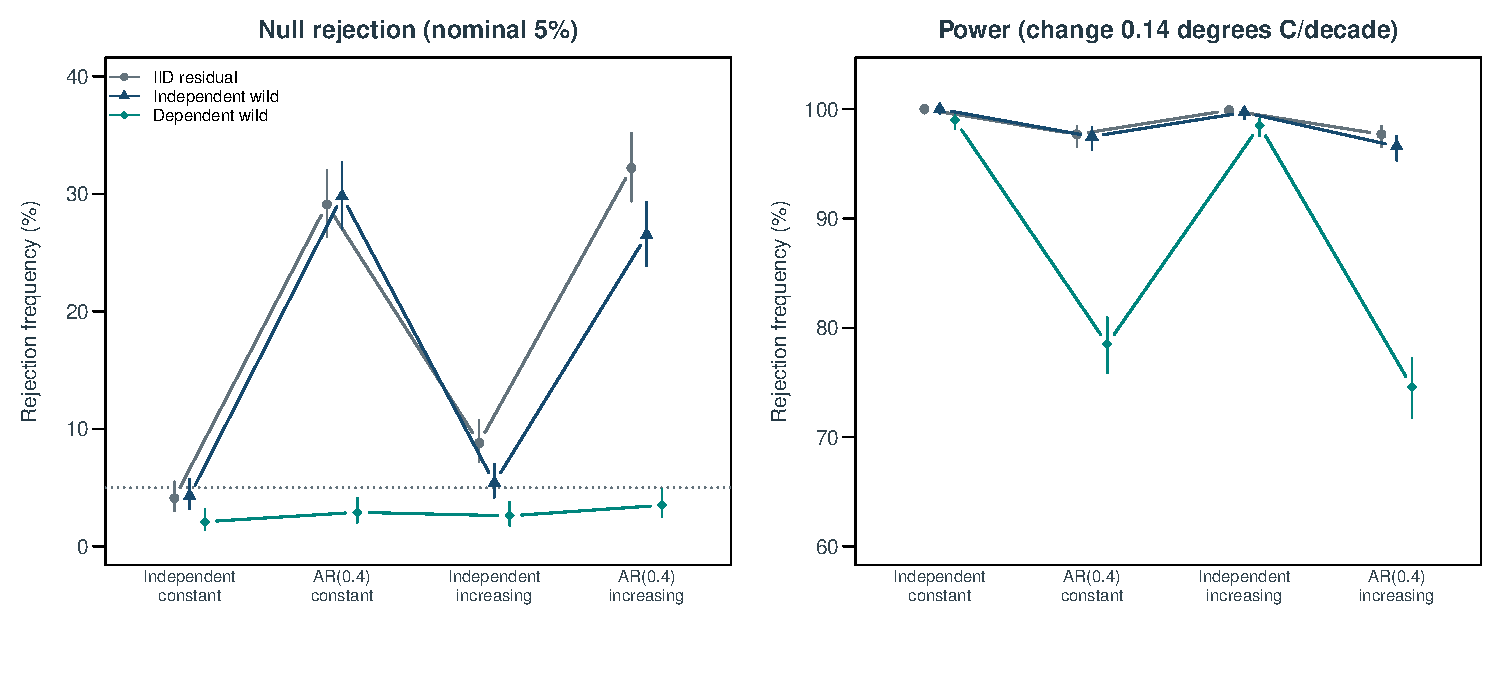
\includegraphics[width=\linewidth]{simulation_results.pdf}
\caption{Size and power across dependence and innovation-scale settings. Vertical intervals are 95\% Wilson intervals for Monte Carlo frequencies. The size panel marks the nominal 5\% level.}\label{fig:sim}\end{figure}

\subsection{Implications and limits}
The experiment supports dependence-aware station inference rather than treating tiny independent-bootstrap $p$-values as decisive. Its cost in these designs is conservatism and lower power. This does not prove the empirical $p$-value is conservative: the observed record has missing years, a different mean history, possible non-Gaussian errors, and unknown dependence. The experiment uses a central, reasonably strong kink, one sample size, and Gaussian innovations. It does not assess weak breaks, other bandwidths, missingness, multiple breaks, or interval coverage. These are focused extensions rather than conclusions established here.

\section{Conclusion}
The complete Station08 record has a positive overall linear slope, but residual diagnostics make a constant trend with independent errors inadequate. A continuous trend with a best-fitting change near 1851 better describes the long-run shape. The fitted later slope is positive and both interval constructions exclude zero; the early slope's intervals contain zero.

Evidence for a statistically identifiable structural break remains qualified: the primary DWB test rejects at 5\%, but a longer bandwidth does not. The date is therefore an uncertain feature of a fitted model rather than an established historical event. The simulation explains why ignoring dependence can exaggerate the evidence. The fitted later slope corresponds to about 0.89\,\degC\ per century; it is an average over the fitted later regime, not a recent-decade rate. The missing decades, measurement history beyond homogenisation, the single-break and dependence specifications, and untested interval coverage limit stronger climate interpretation.

\clearpage\begin{thebibliography}{99}
\bibitem{handout} Friedrich, M. (2026). \emph{Computational Methods in Econometrics: Investigating Temperature Trends: From Linear Trends to Structural Change}. Assignment handout, Vrije Universiteit Amsterdam. Supplied \texttt{CMEAssignment2026Handout.pdf} and \texttt{Station08.csv}.
\bibitem{shao} Shao, X. (2010). The dependent wild bootstrap. \emph{Journal of the American Statistical Association}, 105(489), 218--235. \href{https://doi.org/10.1198/jasa.2009.tm08744}{doi:10.1198/jasa.2009.tm08744}.
\bibitem{friedrich} Friedrich, M., Smeekes, S., and Urbain, J.-P. (2020). Autoregressive wild bootstrap inference for nonparametric trends. \emph{Journal of Econometrics}, 214(1), 81--109. \href{https://doi.org/10.1016/j.jeconom.2019.05.006}{doi:10.1016/j.jeconom.2019.05.006}.
\bibitem{newey} Newey, W. K., and West, K. D. (1987). A simple, positive semi-definite, heteroskedasticity and autocorrelation consistent covariance matrix. \emph{Econometrica}, 55(3), 703--708. \href{https://doi.org/10.2307/1913610}{doi:10.2307/1913610}.
\bibitem{menne} Menne, M. J., Williams, C. N., Gleason, B. E., Rennie, J. J., and Lawrimore, J. H. (2018). The Global Historical Climatology Network Monthly Temperature Dataset, Version 4. \emph{Journal of Climate}, 31(24), 9835--9854. \href{https://doi.org/10.1175/JCLI-D-18-0094.1}{doi:10.1175/JCLI-D-18-0094.1}.
\bibitem{stationdata} NOAA National Centers for Environmental Information. \emph{Global Historical Climatology Network--Monthly Temperature, Version 4}, QCF adjusted series. Supplied \texttt{Station08.csv} and \texttt{Station08\_metadata.pdf}, identifying Geneva and the annual aggregation rule. \href{https://doi.org/10.7289/V5XW4GTH}{Dataset doi:10.7289/V5XW4GTH}.
\bibitem{andrews} Andrews, D. W. K. (1993). Tests for parameter instability and structural change with unknown change point. \emph{Econometrica}, 61(4), 821--856. \href{https://doi.org/10.2307/2951764}{doi:10.2307/2951764}.
\bibitem{wu} Wu, C. F. J. (1986). Jackknife, bootstrap and other resampling methods in regression analysis. \emph{The Annals of Statistics}, 14(4), 1261--1295. \href{https://doi.org/10.1214/aos/1176350142}{doi:10.1214/aos/1176350142}.
\bibitem{liu} Liu, R. Y. (1988). Bootstrap procedures under some non-i.i.d.\ models. \emph{The Annals of Statistics}, 16(4), 1696--1708. \href{https://doi.org/10.1214/aos/1176351062}{doi:10.1214/aos/1176351062}.
\bibitem{davison} Davison, A. C., and Hinkley, D. V. (1997). \emph{Bootstrap Methods and Their Application}. Cambridge University Press, Chapter 5. \href{https://doi.org/10.1017/CBO9780511802843}{doi:10.1017/CBO9780511802843}.
\bibitem{koenker} Koenker, R. (1981). A note on studentizing a test for heteroscedasticity. \emph{Journal of Econometrics}, 17(1), 107--112. \href{https://doi.org/10.1016/0304-4076(81)90062-2}{doi:10.1016/0304-4076(81)90062-2}.
\bibitem{bp} Breusch, T. S., and Pagan, A. R. (1979). A simple test for heteroscedasticity and random coefficient variation. \emph{Econometrica}, 47(5), 1287--1294. \href{https://doi.org/10.2307/1911963}{doi:10.2307/1911963}.
\bibitem{dufour} Dufour, J.-M., and Khalaf, L. (2001). Monte Carlo test methods in econometrics. In B. H. Baltagi (ed.), \emph{A Companion to Theoretical Econometrics}, Chapter 23, 494--519. Blackwell. \href{https://jeanmariedufour.github.io/Dufour_Khalaf_1998_MCTCompanion_W.pdf}{Author manuscript}.
\bibitem{matthews} Matthews, J. A., and Briffa, K. R. (2005). The \textquotedblleft Little Ice Age\textquotedblright: re-evaluation of an evolving concept. \emph{Geografiska Annaler: Series A, Physical Geography}, 87(1), 17--36. \href{https://doi.org/10.1111/j.0435-3676.2005.00242.x}{doi:10.1111/j.0435-3676.2005.00242.x}.
\end{thebibliography}

\clearpage\appendix
\section{Linear-model variance and distribution diagnostics}\label{app:linear-marginal}
\begin{figure}[H]\centering
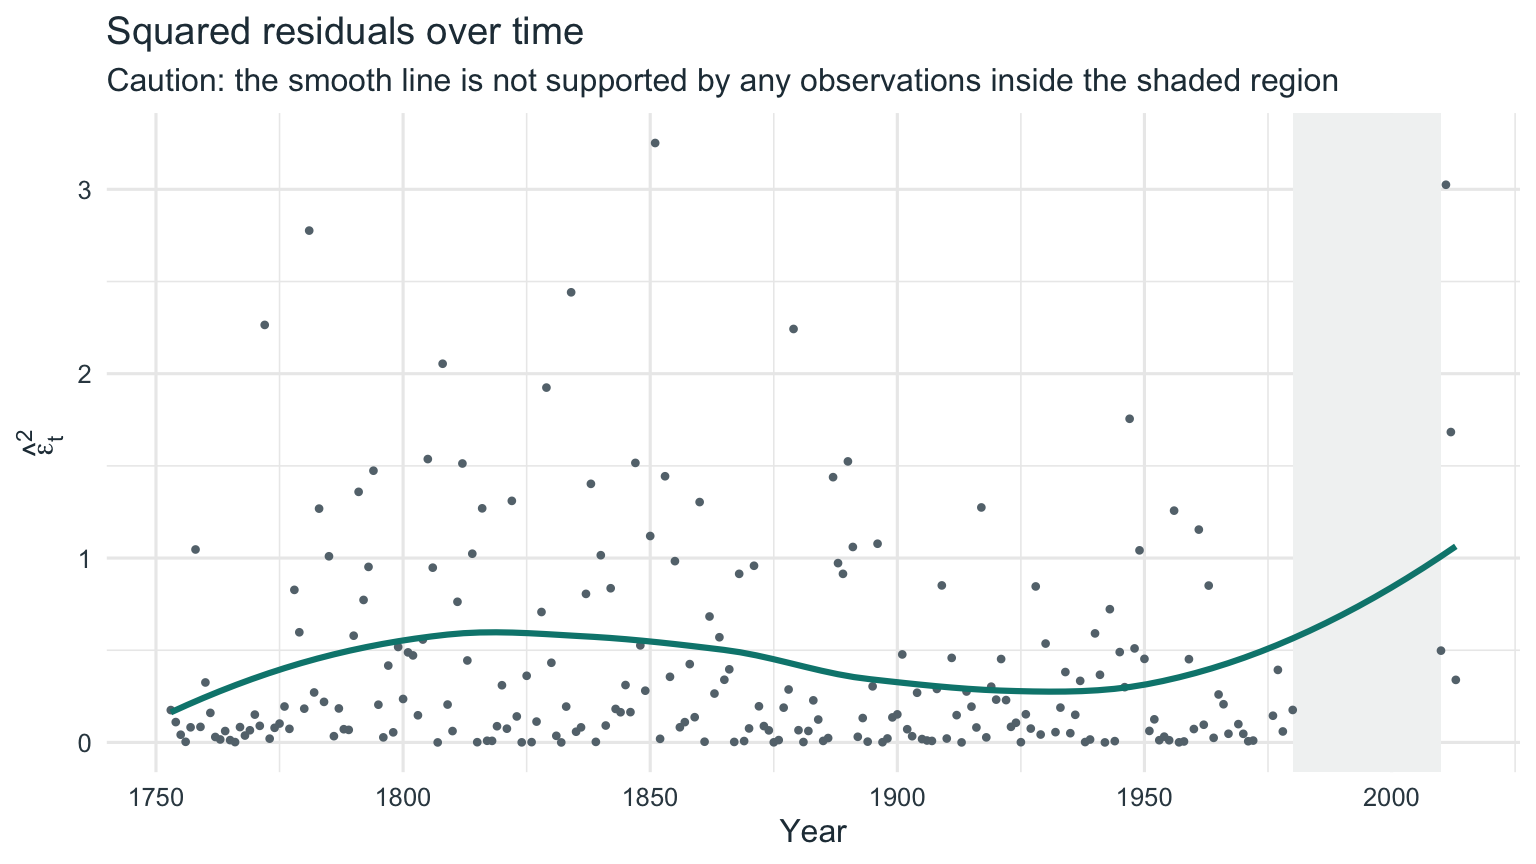
\includegraphics[width=.94\linewidth]{variance-plot-1.png}\\[3mm]
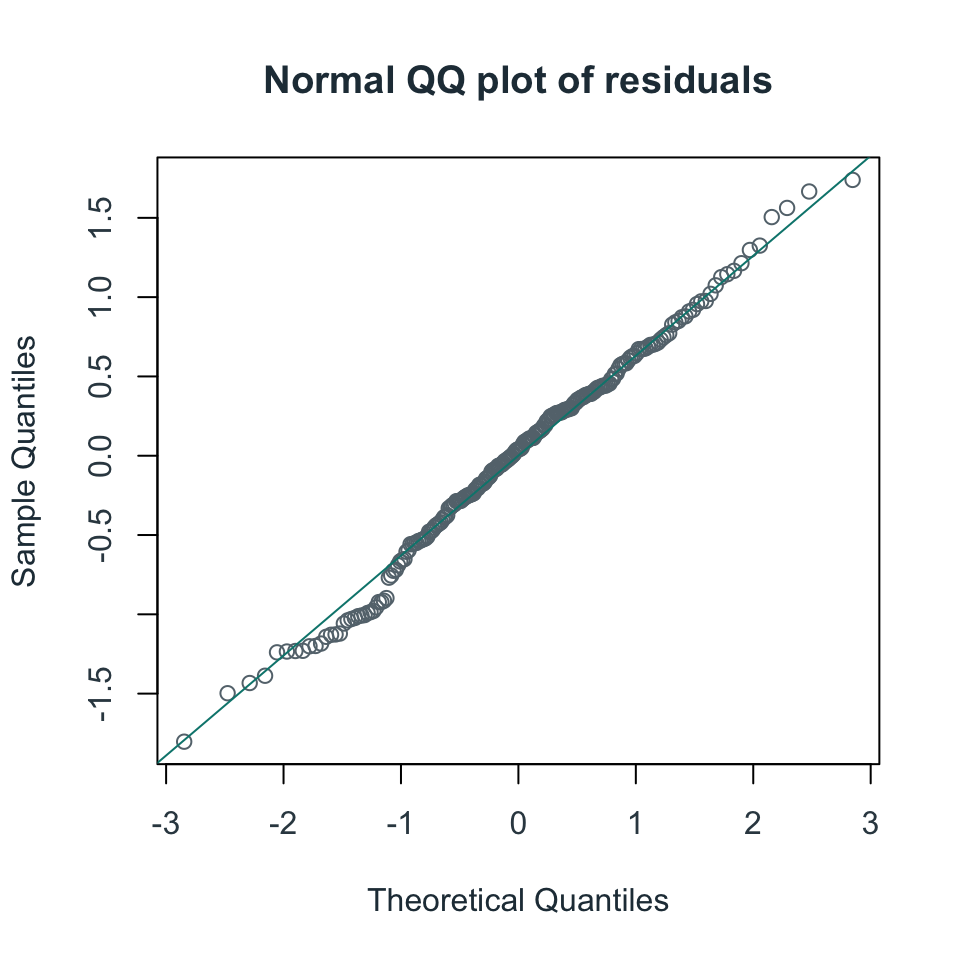
\includegraphics[width=.55\linewidth]{qq-plot-1.png}
\caption{Squared linear-model residuals with a descriptive LOESS smooth (top), and the normal QQ plot (bottom). The smooth does not provide observations inside the shaded gap. The QQ comparison concerns marginal shape and cannot verify independence or constant variance.}
\end{figure}
\section{Supplementary diagnostics and sensitivity}\label{app:diagnostics}
\begin{figure}[H]\centering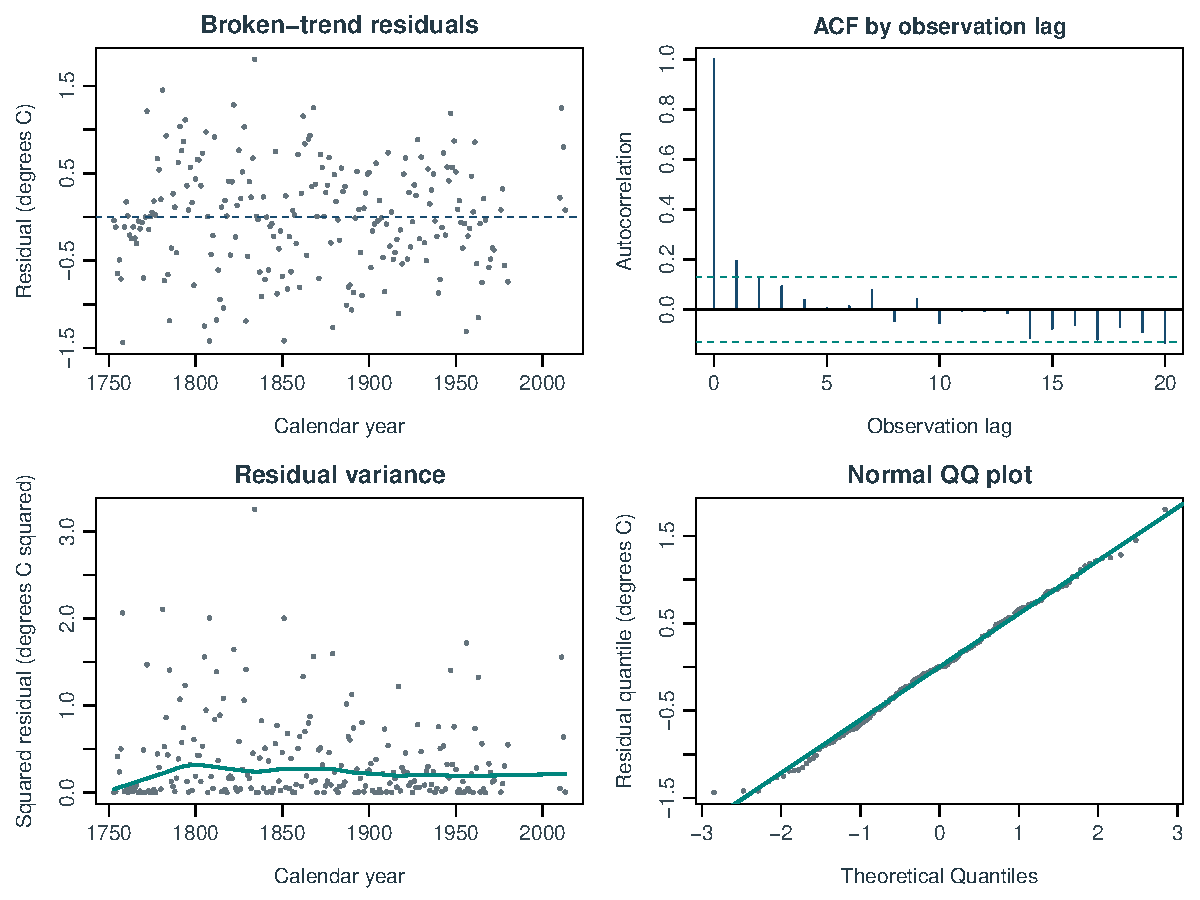
\includegraphics[width=.9\linewidth]{diagnostics_broken.pdf}
\caption{Residual diagnostics after selecting the broken trend. Dependence is reduced but remains visible. ACF lags count observations.}\end{figure}
\begin{table}[H]\centering\small
\caption{Secondary point-estimate sensitivity. Slopes are \degC\ per decade. Each reduced sample reselects the break with 15\% trimming. No bootstrap tests are claimed for these rows.}\begin{tabular}{lrrrrr}
\toprule
Secondary sample & $n$ & Break year & Pre slope & Post slope & $F_T$ \\
\midrule
Omit 1851 & 225 & 1853 & -0.0464 & 0.0872 & 10.982 \\
End in 1980 & 222 & 1850 & -0.0477 & 0.0776 & 8.699 \\
\bottomrule
\end{tabular}
\end{table}
The coldest-observation check removes only 1851; the endpoint check removes only the four 2010--2013 observations. All primary results retain the full sample.

\clearpage\section{Bootstrap null distributions}
\begin{figure}[H]\centering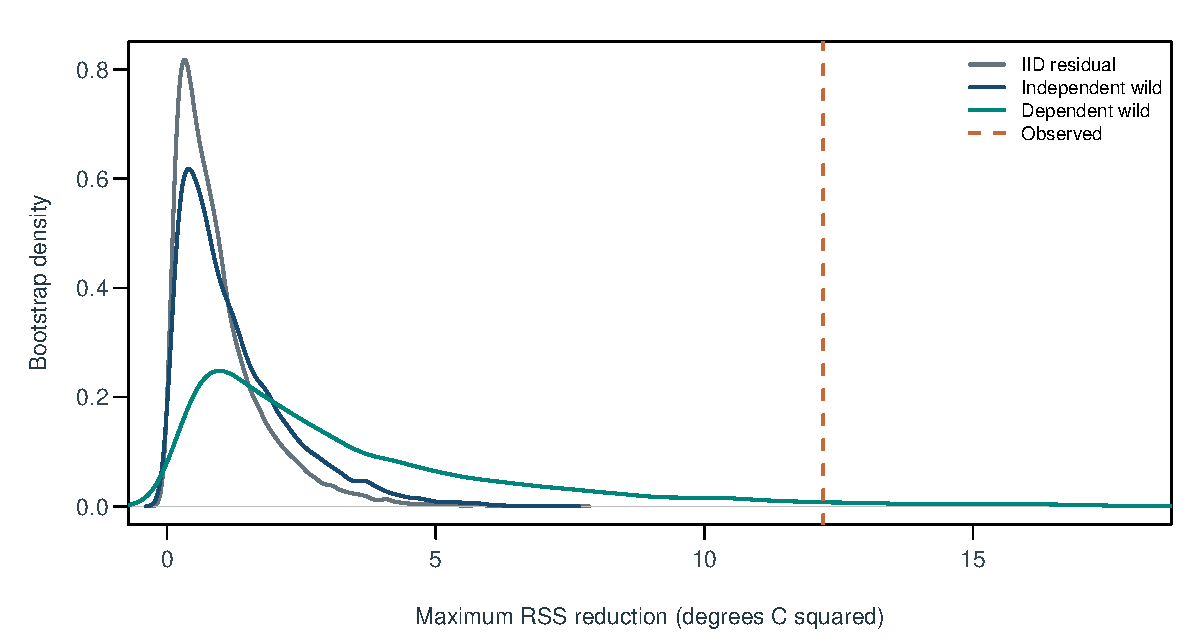
\includegraphics[width=.96\linewidth]{bootstrap_null.pdf}
\caption{Bootstrap null distributions of the maximum RSS reduction. The observed statistic is marked by the dashed line. The dependent wild calibration retains dependence through calendar-indexed multipliers and gives a larger critical value.}
\end{figure}
Every test uses residuals from the linear null, generates data around its fitted mean and repeats the full candidate search. The IID and independent wild results reach the simulation floor; their equality does not resolve smaller tail probabilities or establish that variance patterns are irrelevant.

\clearpage\section{Slope and date variation under the alternative}
\begin{figure}[H]\centering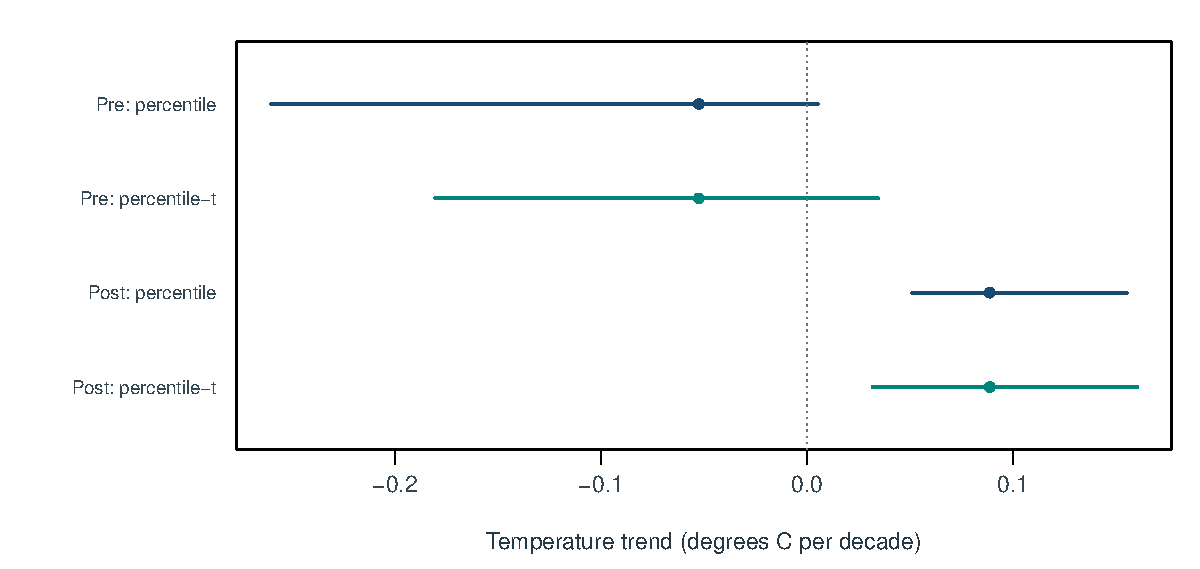
\includegraphics[width=.94\linewidth]{slope_intervals.pdf}
\caption{Percentile and percentile-$t$ slope intervals with zero as a reference.}\end{figure}
\begin{figure}[H]\centering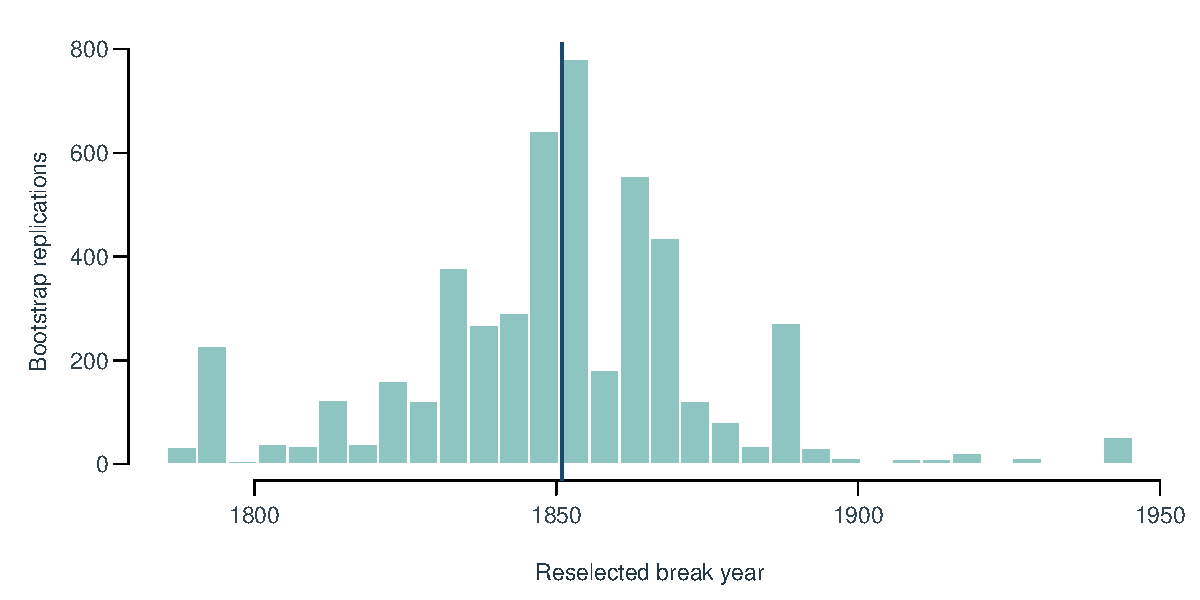
\includegraphics[width=.9\linewidth]{break_bootstrap_distribution.pdf}
\caption{Reselected dates in 4,999 DWB samples under the fitted alternative. The vertical line marks 1851.}\end{figure}
The 2.5th and 97.5th date percentiles are 1793 and 1896; 1.54\% of selections are at trimming boundaries. These summarize variability, rather than form an established 95\% confidence set for a possibly weakly identified break. Date uncertainty helps explain asymmetric slope intervals.

\clearpage\section{Simulation uncertainty and configurations}\label{app:simulation}
\small Configurations 1--2 use independent errors and constant scale; 3--4 use $\rho=0.4$ and constant scale; 5--6 use independent errors and increasing scale; 7--8 use $\rho=0.4$ and increasing scale. Odd configurations have no break; even configurations use $\delta=0.14$.
\begin{table}[H]\centering\footnotesize
\caption{Monte Carlo uncertainty for every result. MC SE is in percentage points. Wilson intervals describe simulation frequencies, not empirical slope uncertainty.}\begin{tabular}{rlrrr}
\toprule
Config. & Procedure & Rejection (\%) & MC SE (pp) & 95\% Wilson interval (\%) \\
\midrule
1 & IID residual & 4.1 & 0.63 & [3.0, 5.5] \\
1 & Independent wild & 4.3 & 0.64 & [3.2, 5.7] \\
1 & Dependent wild & 2.1 & 0.45 & [1.4, 3.2] \\
2 & IID residual & 100.0 & 0.00 & [99.6, 100.0] \\
2 & Independent wild & 100.0 & 0.00 & [99.6, 100.0] \\
2 & Dependent wild & 99.0 & 0.31 & [98.2, 99.5] \\
3 & IID residual & 29.1 & 1.44 & [26.4, 32.0] \\
3 & Independent wild & 29.8 & 1.45 & [27.0, 32.7] \\
3 & Dependent wild & 2.9 & 0.53 & [2.0, 4.1] \\
4 & IID residual & 97.7 & 0.47 & [96.6, 98.5] \\
4 & Independent wild & 97.5 & 0.49 & [96.3, 98.3] \\
4 & Dependent wild & 78.5 & 1.30 & [75.8, 80.9] \\
5 & IID residual & 8.8 & 0.90 & [7.2, 10.7] \\
5 & Independent wild & 5.4 & 0.71 & [4.2, 7.0] \\
5 & Dependent wild & 2.6 & 0.50 & [1.8, 3.8] \\
6 & IID residual & 99.9 & 0.10 & [99.4, 100.0] \\
6 & Independent wild & 99.7 & 0.17 & [99.1, 99.9] \\
6 & Dependent wild & 98.5 & 0.38 & [97.5, 99.1] \\
7 & IID residual & 32.2 & 1.48 & [29.4, 35.2] \\
7 & Independent wild & 26.5 & 1.40 & [23.9, 29.3] \\
7 & Dependent wild & 3.5 & 0.58 & [2.5, 4.8] \\
8 & IID residual & 97.7 & 0.47 & [96.6, 98.5] \\
8 & Independent wild & 96.6 & 0.57 & [95.3, 97.6] \\
8 & Dependent wild & 74.6 & 1.38 & [71.8, 77.2] \\
\bottomrule
\end{tabular}
\end{table}\normalsize

\clearpage\section{Computational reproducibility and validation}\label{app:computation}
The computational source for this report is the refined \texttt{main.Rmd}. It reads \texttt{Station08.csv} relative to its own directory, validates all supplied rows, and writes figures, tables, stored draws, simulation checkpoints and session details under \texttt{work/main\_rmd\_run}. Statistical estimation and resampling use base R and \texttt{parallel}; the document uses \texttt{ggplot2}, \texttt{knitr} and \texttt{rmarkdown}. \texttt{lmtest} supplies optional cross-checks, not the required test implementations. The report uses the Rmd's exported figures and numerical tables; no packaged unknown-break or complete bootstrap command substitutes for the implemented algorithms.

The master seed is 20260926. DW and its QR-based replay use the master seed itself. IID, independent wild and primary DWB break tests use master $+101,+102,+103$; bandwidth checks use master $+203,+212$; CIs use master $+301$. Simulation dataset $m$ in scenario $c$ uses $20260926+100000c+m$, independently of worker scheduling. All reported replication counts were completed. Compatible saved simulation checkpoints avoid repeating an unchanged experiment; the Rmd parameter \texttt{recompute\_simulation = TRUE} requests recomputation.

From the directory containing the refined Rmd and CSV, render with:
\begin{quote}\small\ttfamily
rmarkdown::render("main.Rmd")
\end{quote}
This report compiles from its own directory with \texttt{latexmk -pdf report.tex}; numerical inputs and figure copies are stored in its \texttt{tables/} and \texttt{figures/} subdirectories. The report itself does not rerun the statistics. Session details and validation records are exported by the Rmd.

\subsection{Projection calculation and independent checks}
For a candidate hinge $h_k$, let $v_k=M_Xh_k/\|M_Xh_k\|$. By the Frisch--Waugh--Lovell theorem, the reduction in RSS from adding that hinge is $(v_k'y)^2=(v_k'e_0)^2$. Thus the complete search computes the largest squared projection over the fixed grid. Adding the fitted null mean to bootstrap errors leaves these projections unchanged. The Rmd compares this efficient implementation against explicit OLS at every observed candidate and additional full bootstrap-generated-series fits.

The executable checks also verify:
\begin{itemize}
\item all 226 supplied rows, all five gaps and all 35 absent years; centring invariance of fits and slopes;
\item both 9,999-draw DW reference distributions using an independent QR residual projection, and BP through the squared-correlation identity for its one-regressor auxiliary regression;
\item 21 bootstrap comparisons against explicit null and alternative OLS searches;
\item both slope-interval constructions from all 4,999 stored alternative-bootstrap refits;
\item plus-one empirical p-values, all 8,000 simulation replications, 24 rejection frequencies, Monte Carlo SEs and Wilson intervals;
\item one complete seeded replication from every simulation scenario.
\end{itemize}
These checks address computational consistency; they do not establish bootstrap validity or confidence-interval coverage beyond the assumptions and simulation designs discussed in the main text.

\clearpage\section{Reference year and intercepts}\label{app:centring}
The time variable is $(s_i-1850)/10$. In the linear model, the intercept is fitted temperature in 1850. The fitted break is in 1851, so its hinge is also zero in 1850 and the broken-model intercept has the same reference-year interpretation. At the break, fitted temperature is instead
\[
\widehat y(\widehat T_1)=\widehat\alpha+
\widehat\beta(\widehat T_1-1850)/10.
\]
Changing the reference year only reparametrises the intercept when the hinge date is translated consistently; fitted values, residuals, slopes, the break search and test statistics are invariant. Mean-year centring minimises the classical intercept variance in the simple linear trend model, but no inference here concerns that intercept. The 1850 reference was chosen after seeing the breakpoint for ease of presentation and is not an independently specified climate baseline.

\section{How missing years enter each analysis}\label{app:gaps}
\small
\begin{tabularx}{\linewidth}{@{}p{.20\linewidth}XX@{}}\toprule
Component & Consequence of gaps & Treatment in the Rmd and report\\\midrule
Observed time plots & A connecting line can suggest an unobserved trajectory. & Lines stop across gaps; the largest missing interval is shaded.\\
OLS trend & Coverage affects the estimate and precision. & Actual calendar years and all observations are retained; no imputation.\\
Residual ACF & Observation and calendar lags differ. & Both displayed; the annual grid has NA at absent years, with descriptive bounds.\\
Variance smooth & The curve inside a gap lacks observed support. & Retained as a descriptive smooth with an explicit caveat.\\
QQ plot & Calendar ordering is not part of the construction. & Marginal distribution check, not proof of Gaussianity or independence.\\
DW Monte Carlo & The assigned statistic includes gap-spanning observation pairs. & Standard statistic is primary; the calendar-adjacent variant is separately calibrated.\\
BP diagnostic & Actual time enters algebraically, while dependence affects calibration. & $nR^2$ and nominal $\chi^2_1$ are retained with narrow non-rejection language.\\
Bootstrap inference & Dependence should reflect elapsed time. & DWB multiplier correlation decays with calendar distance; each draw reselects the break.\\
Interpretation & Missing decades and measurement history remain unknown. & No claims about the unobserved trajectory, global change or a physical cause.\\\bottomrule
\end{tabularx}
\normalsize

\end{document}
